\documentclass[12pt]{article}
\usepackage{graphicx} % for including figure 
\usepackage{geometry} % geometry package for mentioning margin length
\usepackage{hyperref}
\usepackage{dirtree}
\usepackage{url}
\usepackage{listings}
%\usepackage{bera}
\usepackage{xcolor}

\geometry{margin=3cm} %for setting margin; DON'T CHANGE THIS
\bibliographystyle{plain}
\usepackage{algorithm}
\usepackage{url}
\usepackage{algpseudocode}
\usepackage[fleqn]{amsmath}
\newcommand{\inlinecode}{\texttt}

\colorlet{punct}{red!60!black}
\definecolor{background}{HTML}{EEEEEE}
\definecolor{delim}{RGB}{20,105,176}
\colorlet{numb}{magenta!60!black}

\lstdefinelanguage{json}{
    basicstyle=\normalfont\ttfamily,
    numbers=left,
    numberstyle=\scriptsize,
    stepnumber=1,
    numbersep=8pt,
    showstringspaces=false,
    breaklines=true,
    frame=lines,
    backgroundcolor=\color{background},
    literate=
     *{0}{{{\color{numb}0}}}{1}
      {1}{{{\color{numb}1}}}{1}
      {2}{{{\color{numb}2}}}{1}
      {3}{{{\color{numb}3}}}{1}
      {4}{{{\color{numb}4}}}{1}
      {5}{{{\color{numb}5}}}{1}
      {6}{{{\color{numb}6}}}{1}
      {7}{{{\color{numb}7}}}{1}
      {8}{{{\color{numb}8}}}{1}
      {9}{{{\color{numb}9}}}{1}
      {:}{{{\color{punct}{:}}}}{1}
      {,}{{{\color{punct}{,}}}}{1}
      {\{}{{{\color{delim}{\{}}}}{1}
      {\}}{{{\color{delim}{\}}}}}{1}
      {[}{{{\color{delim}{[}}}}{1}
      {]}{{{\color{delim}{]}}}}{1},
}


\title{Project documentation}
\author{Lorenzo Zanolin}

\begin{document}
\maketitle

\section{Introduction}
The aim of this project is the study of Yao's protocol \cite{yao} and an useful application of it. More precisely, we will implement Secure multi-party computation; this field has the goal of creating methods for parties to jointly compute a function over their inputs while keeping those inputs private \cite{mpc}. In this project, the function we decided to implement is the \textit{8 bit sum}.

\section{Analysis}
We can focus on the sum computed by two parties, say Alice and Bob. The goal is to use \textit{MPC} to calulate the result while avoiding each member to know the others values; to do that we need an external component, called \textit{OT}.\\ This protocol allows two parties, Alice who
knows x and Bob who knows y, to compute jointly the value of $f(x, y)$ in a way that does not reveal to each side more information than can be deduced from $f(x, y)$ \cite{ot}. As already written, $f$ is the 8-bit sum.\\ Both Alice and Bob have a set of integers and need to compute the sum of everything.
Two new roles are introduced: Alice is the \textit{garbler} and has the responsibility of creating the garbled circuit, while Bob is the \textit{evaluator}.
They will behave as follows:
\begin{enumerate}\label{behaviour}
    \item Alice creates the garbled circuit and the tables and send them to Bob.
    \item Alice select her set, via input.
    \item Bob select his set, via input.
    \item Both interact with each other using OT.
    \item Bob evaluate the function result and sends it to Alice.
    \item Alice checks the correctness of the result, and sends it to Bob (in clear).
\end{enumerate}

\section{Implementation}
We will present how to implement the \textit{circuit} and how to make Alice and Bob comunicate securely.
\subsection{Circuit}
We will present briefly the 8-bit sum circuit. There are three basic components in this construction:
\begin{itemize}
    \item \textit{\hyperref[half]{Half Adder}}: used to sum the right-most digit;
    \item \textit{\hyperref[full]{Full adder}}:  used to sum a generic digit in the number, ranging from position 1 to 8. It receives in input also carry of the previous sum.
    \item \textit{\hyperref[overflow]{If then else}}: there could be situations, called \textit{overflow}, in which you sum two number with the same sign and obtain a number with opposite sign; to avoid this scenario, this construct is employed by examining the signs of the two numbers and the sign of the calculated result. If the two input numbers have the same sign, the output sign is set to be the same as the inputs. Instead, if the two input numbers have different signs, the sign of the result is determined accordingly to the previous circuit.  
\end{itemize}

\begin{figure}[!htb]
    \begin{center}
        \begin{minipage}{0.4\textwidth}
            \centering
            
\includegraphics[width=.7\linewidth]{../src/images/Half_adder.png}
            \caption{Half Adder}\label{half}
        \end{minipage}
        \hfill
        \begin{minipage}{0.4\textwidth}
            \centering
            
\includegraphics[width=.8\linewidth]{../src/images/Full-adder.png}
            \caption{Full Adder}\label{full}
        \end{minipage}
        \hfill
        \begin{minipage}{0.5\textwidth}
            \centering
            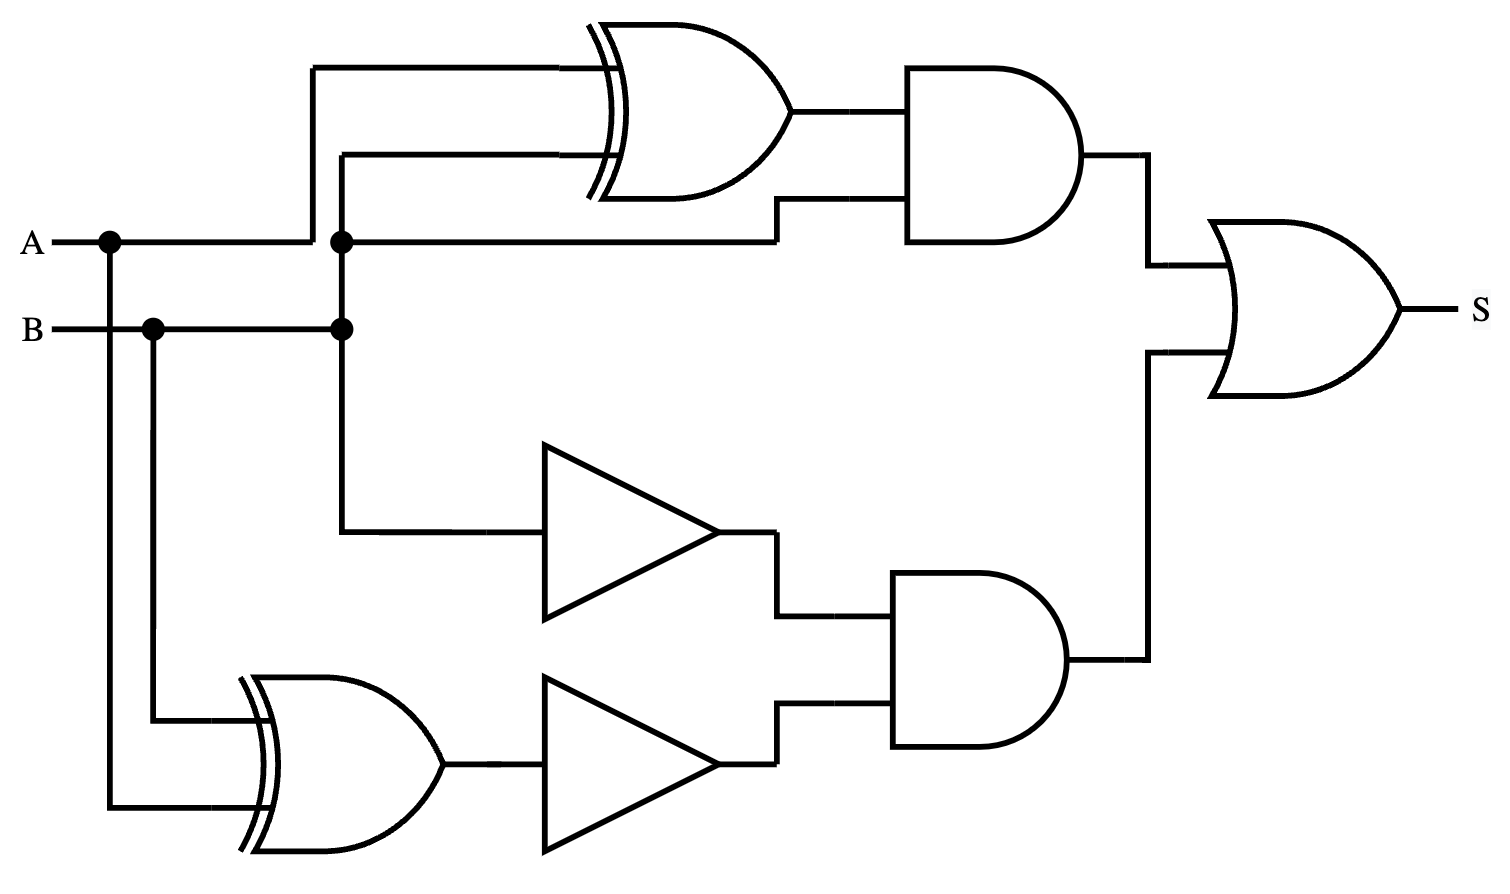
\includegraphics[width=1.2\linewidth]{../src/images/overflow.png}
            \caption{If then else}\label{overflow}
        \end{minipage}
    \end{center}
\end{figure}

\footnote{\ref{half} was taken over \url{https://upload.wikimedia.org/wikipedia/commons/1/14/Half-adder.svg} 
\ref{full} was taken over \url{https://upload.wikimedia.org/wikipedia/commons/a/a9/Full-adder.svg}.}

We then proceede creating the circuit by wiring 7 full adders, an half adder and the if-then-else together, as represented in Figure \ref{circuit}.

\begin{figure}[!h]
    %\centering
    \makebox[\textwidth][c]{
    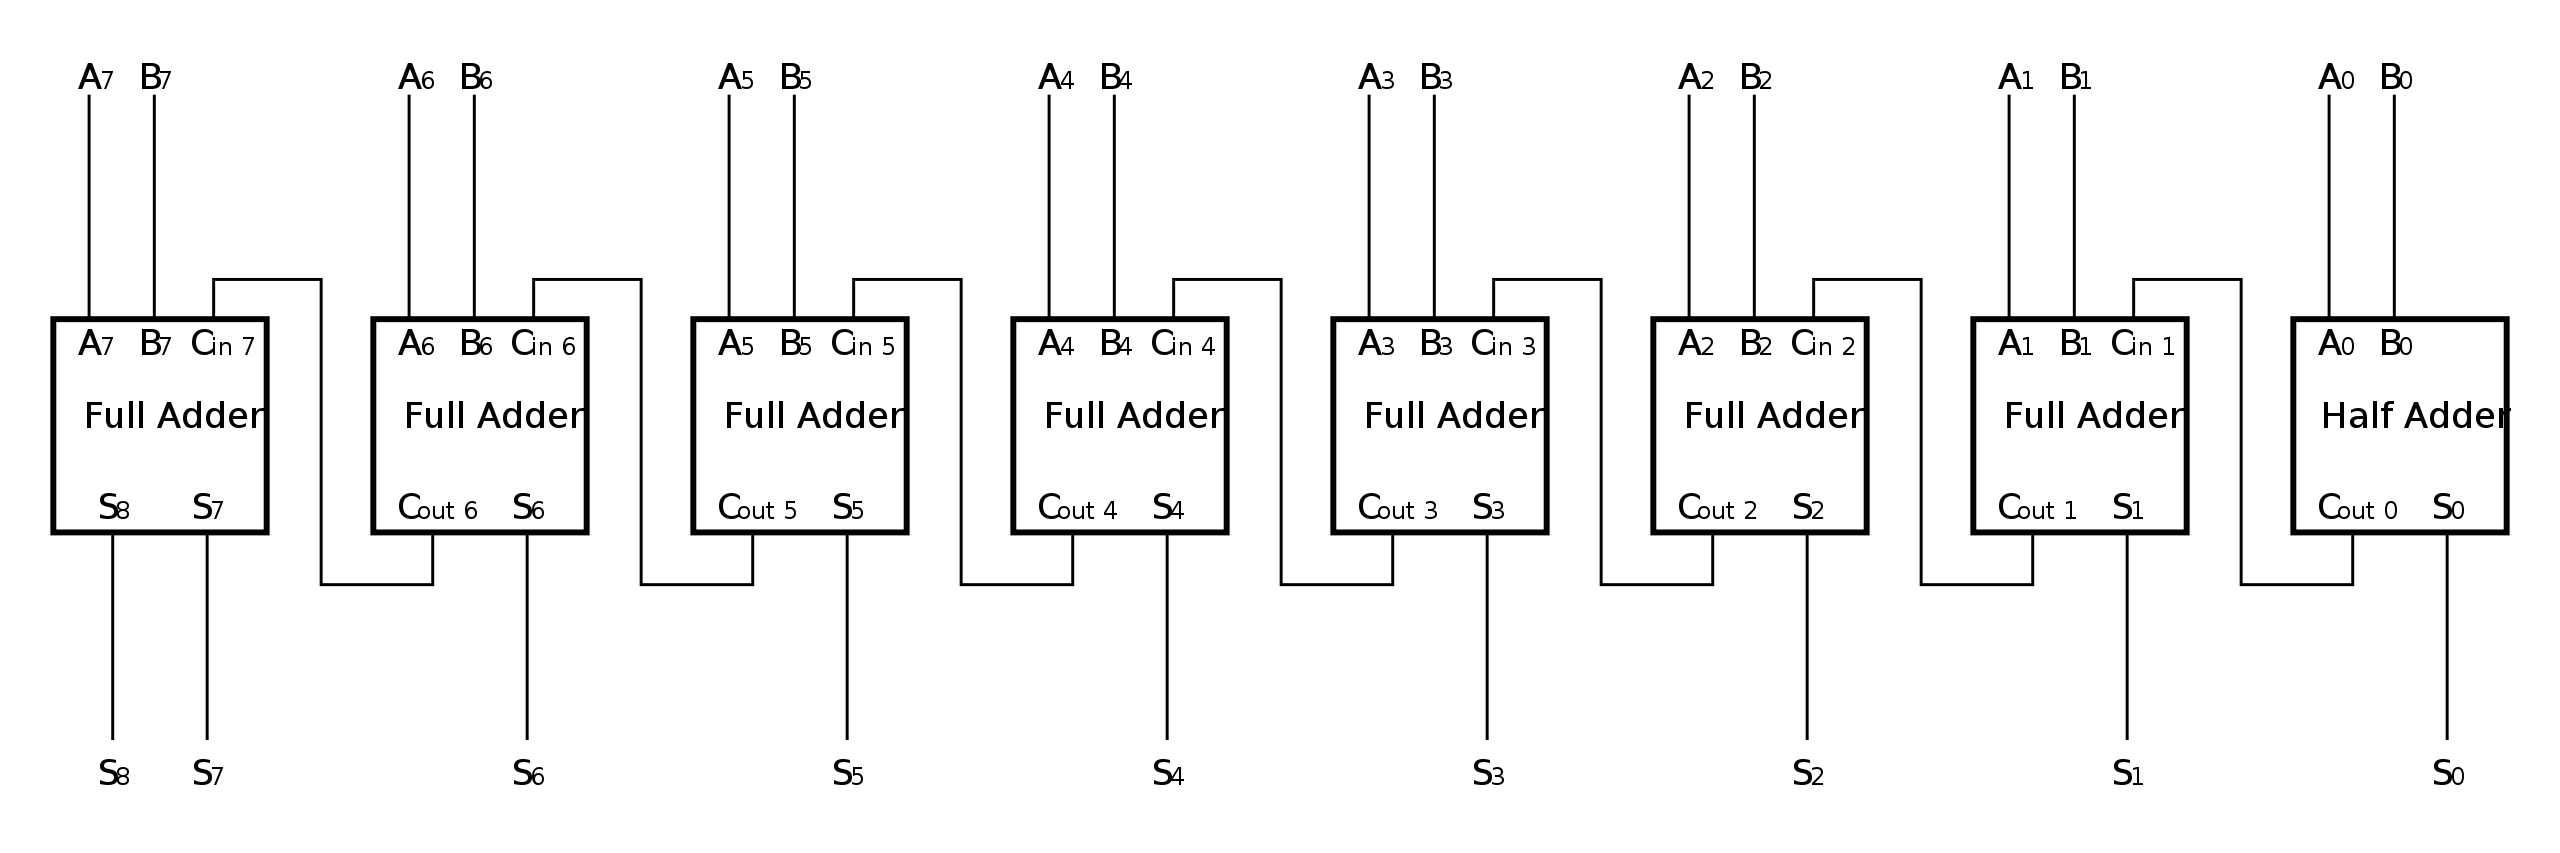
\includegraphics[width=1.2\linewidth]{../src/images/Circuit.png}}
    \caption{8-bit Adder}\label{circuit}
\end{figure}
Since we are using 8 bit to represent the sum of each set, it immediatly follows that the sum of each set must be smaller than 256. In this case we are dealing with \textit{integers}, thus we also need to consider negative numbers; to do that we are using \textit{2-complement}. In this case we are considering numbers that belong to [-128,127]. The final sum has 9 bit representation, thus the result that we can obtain belongs to [-256,254]. 
%\subsection{Implementation}
\subsubsection{Project structure}
The project will be developed using \textit{Python 3.9.10} and we will use functions provided in the GitHub repo \url{https://github.com/ojroques/garbled-circuit}\label{ref:git}.\\
There is also a dedicated GitHub page related to this project at \url{https://github.com/lorenzozanolin/garbledCircuit}\label{zanoGit}.\\ \\ The project has the following structure:\\ \\
The \inlinecode{code} folder contains all the file that we will utilize for the secure communication. \inlinecode{ot.py, util.py, yao.py} are utilities taken from \hyperref[ref:git]{Ojroques repo}.\\
The \inlinecode{images} folder contains all images used in the report and documentation.\\
The \inlinecode{circuits} folder contains the used circuit, in this case only \inlinecode{add.json}\\
The \inlinecode{sets} folder contains the two files used to store sets of Alice and Bob.\\
\fbox{
    \begin{minipage}{40em}
    \dirtree{%
    .1 src/..
    .2 Makefile.
    .2 images \hspace{5cm} \begin{minipage}[t]{10cm}
        This directory contains the images used{.}
        \end{minipage}.
    .3 {...}.
    .2 circuits \hspace{4.5cm} \begin{minipage}[t]{10cm}
        This directory contains the circuit used{.}
        \end{minipage}.
    .3 add.json.
    .2 code \hspace{5cm} \begin{minipage}[t]{10cm}
        This directory contains the code used{.}
        \end{minipage}.
    .3 util.py.
    .3 yao.py.
    .3 ot.py.
    .3 requirements.py.
    .3 main.py.
    .2 sets \hspace{5cm} \begin{minipage}[t]{10cm}
        This directory contains the sets saved{.}
        \end{minipage}.
    .3 alice.txt.
    .3 bob.txt.
    }
    \end{minipage}
}\\ \\

\subsubsection{Coding part}
First thing first, we need to represent the \textit{circuit}; we decided to create the \inlinecode{add.json} file to code the circuit. Each wire is mapped to a number and linked with the other following the structure represented in Figure \ref{circuit}.\\* Each gate that appears in figure \ref{circuit} is represented in a single JSON line.\\*
The syntax is:\\ \\
\fbox{\inlinecode{"id" : <gateId>, "type" : "<TYPE>", "in": [<gateIdInput1>, <gateIdInput2>]}}\\ \\
In this case the circuit is represented as follows:
\begin{lstlisting}[language=json,firstnumber=1]
    {"name":"adder",
     "circuits":[
      {
        "id":"8 bit adder",
        "alice":[47,40,33,26,19,12,5,1],
        "bob":[48,41,34,27,20,13,6,2],
        "out":[62,50,43,36,29,22,15,8,3],
        "gates":[
            {"id":3,"type":"XOR","in":[1,2]},
            {"id":4,"type":"AND","in":[1,2]},

            {"id":7,"type":"XOR","in":[5,6]},
            {"id":8,"type":"XOR","in":[4,7]},
            {"id":9,"type":"AND","in":[4,7]},
            {"id":10,"type":"AND","in":[5,6]},
            {"id":11,"type":"OR","in":[9,10]},

            {"id":14,"type":"XOR","in":[12,13]},
            {"id":15,"type":"XOR","in":[11,14]},
            {"id":16,"type":"AND","in":[11,14]},
            {"id":17,"type":"AND","in":[12,13]},
            {"id":18,"type":"OR","in":[16,17]},
            
            {"id":21,"type":"XOR","in":[19,20]},
            {"id":22,"type":"XOR","in":[18,21]},
            {"id":23,"type":"AND","in":[18,21]},
            {"id":24,"type":"AND","in":[19,20]},
            {"id":25,"type":"OR","in":[23,24]},
            
            {"id":28,"type":"XOR","in":[26,27]},
            {"id":29,"type":"XOR","in":[25,28]},
            {"id":30,"type":"AND","in":[25,28]},
            {"id":31,"type":"AND","in":[26,27]},
            {"id":32,"type":"OR","in":[30,31]},
            
            {"id":35,"type":"XOR","in":[33,34]},
            {"id":36,"type":"XOR","in":[32,35]},
            {"id":37,"type":"AND","in":[32,35]},
            {"id":38,"type":"AND","in":[33,34]},
            {"id":39,"type":"OR","in":[37,38]},
            
            {"id":42,"type":"XOR","in":[40,41]},
            {"id":43,"type":"XOR","in":[39,42]},
            {"id":44,"type":"AND","in":[39,42]},
            {"id":45,"type":"AND","in":[40,41]},
            {"id":46,"type":"OR","in":[44,45]},
            
            {"id":49,"type":"XOR","in":[47,48]},
            {"id":50,"type":"XOR","in":[46,49]},
            {"id":51,"type":"AND","in":[46,49]},
            {"id":52,"type":"AND","in":[47,48]},
            {"id":53,"type":"OR","in":[51,52]},
            
            {"id":54,"type":"AND","in":[47,48]},
            {"id":55,"type":"NOT","in":[47]},
            {"id":56,"type":"NOT","in":[48]},
            {"id":57,"type":"AND","in":[55,56]},
            {"id":58,"type":"OR","in":[54,57]},
            {"id":59,"type":"AND","in":[47,58]},
            {"id":60,"type":"NOT","in":[58]},
            {"id":61,"type":"AND","in":[50,60]},
            {"id":62,"type":"OR","in":[59,61]}
        ]}]}
    \end{lstlisting}
We then created \inlinecode{class Alice, class Bob} in \inlinecode{main.py} to represent their behaviour.
It was decided that both parties have command line user interaction with the user, so we developed \inlinecode{askForInput} in \inlinecode{requirements.py}. In the same file we can also find two functions \inlinecode{saveSet, readSet} used to write in two external files \inlinecode{sets/alice.txt} and \inlinecode{sets/bob.txt} the input values; this will be useful when we want to check the correctness of the computed result, using \inlinecode{verifyOperation}.\\
Since the communication is encrypted, we decided to use \textit{AES-CBC} as technique; we can see that in the file \inlinecode{yao.py}, more precisely in the two functions \inlinecode{encrypt, decrypt}. As written in the code, we opted to prepend the IV at the cyphertext to avoid reusing the same IV for all the communications.\\
We can represent the pseudocode that represents the behaviour listed before.\\

\begin{minipage}{0.46\textwidth}
    \begin{algorithm}[H]
        \centering
        \caption{Alice's behaviour}\label{alice:algo}
        \begin{algorithmic}[1]
            \State $send(circuit)$  
            \State $aliceSet \gets askForInput()$ 
            \State $saveSet(aliceSet)$ 
            \State
            \State $aliceValue \gets sum(aliceSet)$
            \State $aliceE \gets encrypt(aliceValue)$
            \State
            \State $r \gets OT.getResult(aliceE,bKeys)$
            \State
            \State $result = decimal(r)$
            \State $msg \gets verifyOperation(result)$ 
            \State $sendToBob(msg)$
            \State $printResult(result,msg)$

        \end{algorithmic}
    \end{algorithm}
    \end{minipage}
    \hfill
    \begin{minipage}{0.46\textwidth}
    \begin{algorithm}[H]
        \centering
        \caption{Bob's behaviour}\label{bob:algo}
        \begin{algorithmic}[1]
            \State $receive(circuit)$  
            \State $bobSet \gets askForInput()$ 
            \State $saveSet(bobSet)$ 
            \State
            \State $bobValue \gets sum(bobSet)$
            \State
            \State $OT.sendResult(bobValue)$
            \State
            \State $msg \gets receive()$
            \State $printResult(msg)$

        \end{algorithmic}
    \end{algorithm}
    \end{minipage}

\section{Usage}
We will briefly explain how to install the program and how it works. In my \hyperref[zanoGit]{repo} there is also a graphical visualization of the executing program. 
\subsection{Installation}
To run the program you need some packages:
\begin{itemize}
    \item \textit{ZeroMQ} used in \inlinecode{util.py} to implement communication;
    \item \textit{SymPy} to use prime numbers;
    \item \textit{AES} from encryption;
    \item \textit{Bits} from bitstring, to do conversions from 2-complement to integers.
\end{itemize}
Simply run: 
\inlinecode{\$ pip3 install pyzmq sympy cryptography bitstring}
\subsection{Execution}
As already writte, there are two parties: Alice and Bob. You must run on two different terminals them. From now, for simplicity, we assume that we are positioned inside \inlinecode{/src/}.
From Alice's Terminal, simply run \inlinecode{make alice}, while for Bob's Terminal run run \inlinecode{make bob}.\\
Now the connection will be established and the program will ask the user to give the input set, for each party. Once done, the result will be computed and printed in each terminal.
\subsubsection{Example}
A practical example will follow, we will show the output of each terminal.\\
\textbf{Alice' side}:
\begin{lstlisting}[frame=single, basicstyle=\scriptsize]
$ make alice
python3 code/main.py alice   -c circuits/add.json
Enter the list of integers of Alice's set: 1 2 -5
[1, 1, 1, 1, 1, 1, 1, 0]

======== 8 bit adder ========

Values of the computation

Syntax: parties/result:  [list of bits] = [correspective values]

Alice: [8, 7, 6, 5, 4, 3, 2, 1] = 1 1 1 1 1 1 1 0
Computed result by circuit: [53, 51, 46, 41, 36, 31, 26, 21, 17] = 1 1 1 1 1 1 0 0 0

The sum has been done correctly, result is -8.
\end{lstlisting}
\textbf{Bob's side}:
\begin{lstlisting}[frame=single, basicstyle=\scriptsize]
$ make bob
python3 code/main.py bob
Enter the list of integers of Bob's set: 4 6 -16
Received 8 bit adder
[1, 1, 1, 1, 1, 0, 1, 0]

Syntax:  parties/result  [list of bits] = [correspective values]

Bob [16, 15, 14, 13, 12, 11, 10, 9] = 1 1 1 1 1 0 1 0


The sum has been done correctly, result is -8.
\end{lstlisting}
\textit{Interpretation}: As already written in the output, the syntax is\\ \inlinecode{parties/result:  [list of bits] =   [correspective values]}. \vspace{2mm} \\
The numbers on the left represent the bits in the circuit \inlinecode{add.json}, while the right ones represent the corrispective values. The last line is the output of the function \inlinecode{verifyOperation}.


\bibliography{thud}
\end{document}